
\documentclass[12pt]{article}
\usepackage{amsmath, amssymb, geometry, fancyhdr}
\usepackage{MnSymbol,wasysym}
\geometry{a4paper, margin=1in}
\setlength{\headheight}{15pt}
\pagestyle{fancy}
\fancyhf{}
\fancyhead[L]{CSCI-769 Quantum Computing Principles and Applications}
\fancyhead[R]{}
\fancyfoot[C]{\thepage}
\newcommand{\bra}[1]{\langle #1 |}
\newcommand{\ket}[1]{| #1 \rangle}
\usepackage{xcolor}
\usepackage{hyperref}
\usepackage{piton}
\usepackage{quantikz}
\usepackage{listings}

\lstset{
    language=Python,
    basicstyle=\ttfamily\small,
    keywordstyle=\color{blue},
    commentstyle=\color{green},
    stringstyle=\color{red},
    numbers=left,
    numberstyle=\tiny\color{gray},
    frame=single,
    breaklines=true,
    captionpos=b
}

\begin{document}

\title{CSCI-769 Quantum Computing Principles and Applications Homework 5}
\author{}
\date{}
\maketitle

\subsection*{1) Shor's Algorithm (100 pts)}
\textbf{Summary}: Shor's algorithm is fascinating because it showcases the power of quantum computers to efficiently solve problems that classical computers find exceedingly difficult. Specifically, Shor's algorithm targets the integer factoring problem, where the goal is to find the prime factors of a given integer. Classical computers solve this problem inefficiently; as numbers grow larger, factoring them requires exponentially increasing computational resources, quickly becoming impractical.

Quantum computers utilizing Shor's algorithm achieve an exponential speed-up by cleverly harnessing quantum phenomena such as superposition, interference, and entanglement. The algorithm works by transforming the factoring problem into the task of identifying the period of a certain mathematical function (modular exponentiation). This period-finding step is efficiently performed using the Quantum Fourier Transform (QFT). After identifying the period, factoring the integer itself becomes relatively straightforward.

Unlike algorithms such as Deutsch-Jozsa, which address artificial computational problems without direct practical importance, Shor's algorithm solves a genuinely important mathematical problem. Moreover, Shor's success suggests that other complex problems might possess hidden structures exploitable by quantum algorithms, offering hope that quantum computing could revolutionize problem-solving across diverse computational domains. In this exploration, you will examine Shor's algorithm in detail, understanding its quantum circuit structure, how the Quantum Fourier Transform is utilized, and the transformation from abstract algorithms into concrete circuit implementations.

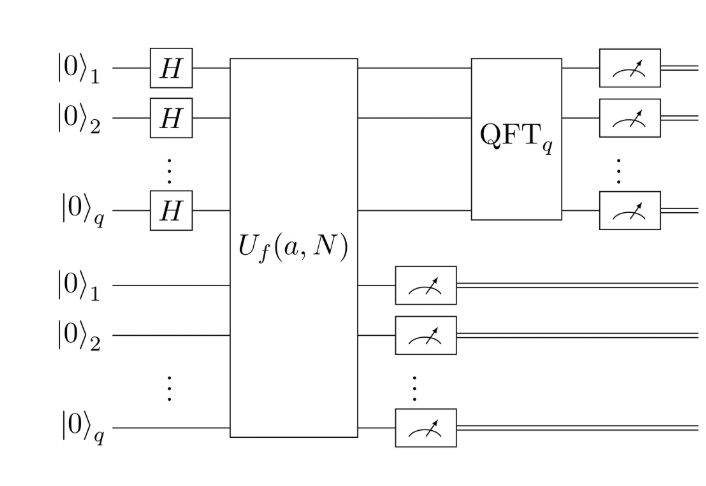
\includegraphics[scale=.75]{shorpng.png}

\begin{itemize}
   \item Consider Shor's circuit above:
   \begin{itemize}
      \item Execute the circuit with parameters $N=15$ and $a=2$ on the quantum simulator. Record the determined period and consequently identify the prime factors.
       \item Execute the circuit with parameters $N=35$ and $a=2$. Record the determined period and consequently identify the prime factors.
   \end{itemize}

    \item Although we won't be executing this on a NISQ device because many individuals have exhausted their available time on IBM machines \smiley{}, let's delve into the concept. Analyze the circuit's depth and width as $N$ approaches infinity. Could Shor's algorithm be successfully executed on a NISQ for a large $N$, given a sufficient number of physical qubits? Discuss whether this is feasible or not, and if it is not, suggest potential solutions to support the factoring algorithm.

\end{itemize}







\subsection*{Bonus 1: HHL Algorithm (50 pts)}
Summary: The Harrow-Hassidim-Lloyd (HHL) algorithm is remarkable because it demonstrates the potential of quantum computers to efficiently solve linear systems of equations—a fundamental task prevalent in scientific computing, engineering, and data analysis. Classical methods, such as Gaussian elimination or iterative techniques, typically scale poorly with large matrices, quickly becoming impractical for very large systems.

Quantum computers, using the HHL algorithm, offer an exponential speed-up for solving certain linear systems by exploiting quantum properties like superposition and entanglement. Specifically, the HHL algorithm transforms the classical problem of solving a linear equation $Ax=b$ into a quantum state preparation and measurement problem. It utilizes phase estimation and Hamiltonian simulation to encode solutions efficiently into quantum states.

Unlike abstract quantum algorithms designed primarily as theoretical demonstrations, HHL addresses a practically relevant computational challenge. Its success provides evidence that quantum algorithms can efficiently handle structured mathematical problems, raising hope that quantum computing may similarly accelerate solutions across other computational domains. In your exploration, you'll dive into the quantum circuit implementation of HHL, examine the role of quantum subroutines like phase estimation, and understand how theoretical oracle-based representations can be translated into explicit quantum circuit implementations.\smiley{}.

For each linear system - identify the solution to the linear equation(s) and then implement the HHL algorithm to solve it (Hint: Determine what $A$ and $b$ are in each instance): 

 a) $x_1=1$ (one unknown)
    
    b) \begin{align*}
        &x_1-x_2=-1\\
        &x_1+x_2=1
    \end{align*}
    (two unknowns)


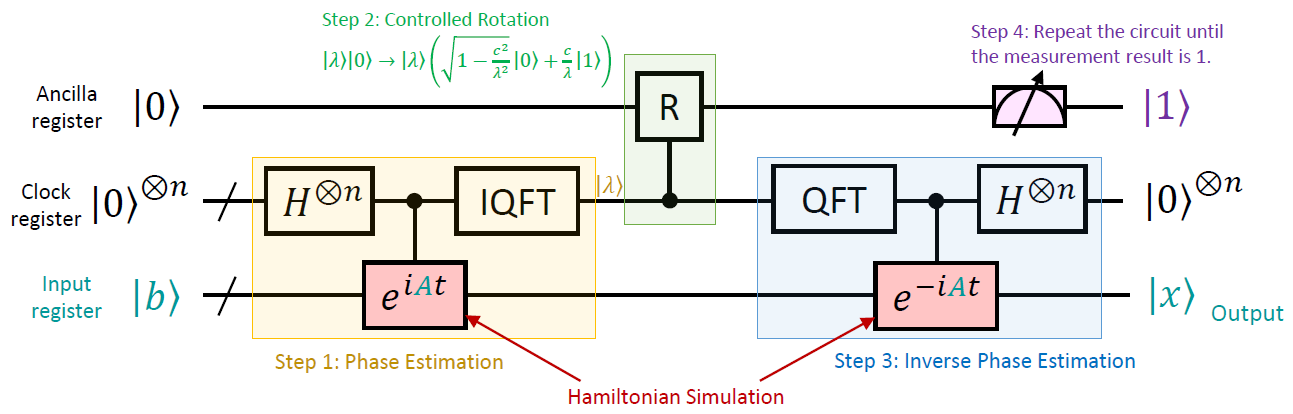
\includegraphics[scale=.4]{hhl.png}

\subsection*{Bonus 2: QAOA Algorithm (50 pts)}
Summary: The Quantum Approximate Optimization Algorithm (QAOA) is intriguing because it represents a practical, near-term quantum algorithm designed for solving combinatorial optimization problems—tasks that appear frequently in logistics, resource allocation, and network design. These problems typically involve finding the optimal solution among an enormous number of possibilities, a task classical computers struggle with due to rapidly increasing complexity.

Quantum computers utilizing QAOA aim to efficiently approximate optimal solutions by combining quantum and classical computational techniques. QAOA operates by iteratively applying parameterized quantum gates designed to encode the optimization problem and then using classical optimization methods to fine-tune these parameters. Through the interplay of quantum properties such as superposition and interference, QAOA explores solution spaces more effectively than classical heuristics.

What makes QAOA particularly exciting is its immediate relevance and adaptability to today's noisy, intermediate-scale quantum (NISQ) devices. Unlike many purely theoretical quantum algorithms requiring extensive fault-tolerance, QAOA can be implemented on current and near-term quantum hardware. This practicality provides hope that quantum computers will soon deliver tangible advantages for complex optimization problems. In this exploration, you will delve into the structure and implementation of QAOA, examine how quantum circuits encode specific optimization problems, and explore the interaction between classical and quantum computations in achieving optimal performance.

Examine the circuit below along with the optimization problem presented:
\begin{align}
    \underset{x}{\text{minimize}} \sum_{i=1}^{N} x_i^2 \\
    x_i \in \{0,1\}
\end{align}
a)Determine the minimum solution for this objective function. Is this a globally minimal solution, and why?\smiley{}.
b)Determine a circuit implementation for the case when $N=10$ using $p=1,5,10$. Begin with all $\gamma_i$ and $\beta_i$ initialized to 1, updating the parameters through gradient descent at the conclusion of each iteration. Identify the number of QAOA iterations needed to reach the global minimum for each value of $p$ (did convergence occur?). Discuss the general trend in the number of iterations QAOA that are needed in solving the optimization problem relative to the parameter $p$. With increasing $p$, consider the challenges that may arise for NISQ systems and how these can be mitigated using error correction techniques. For details on $H_c$, refer to the lecture notes, taking into account that, given binary variables, $x_i^2=x_i$.

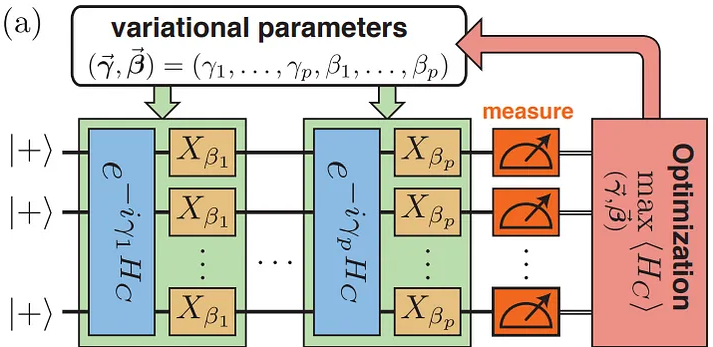
\includegraphics[scale=.75]{qaoapng.png}
\end{document}


\end{document}
